% This file was created with tikzplotlib v0.10.1.
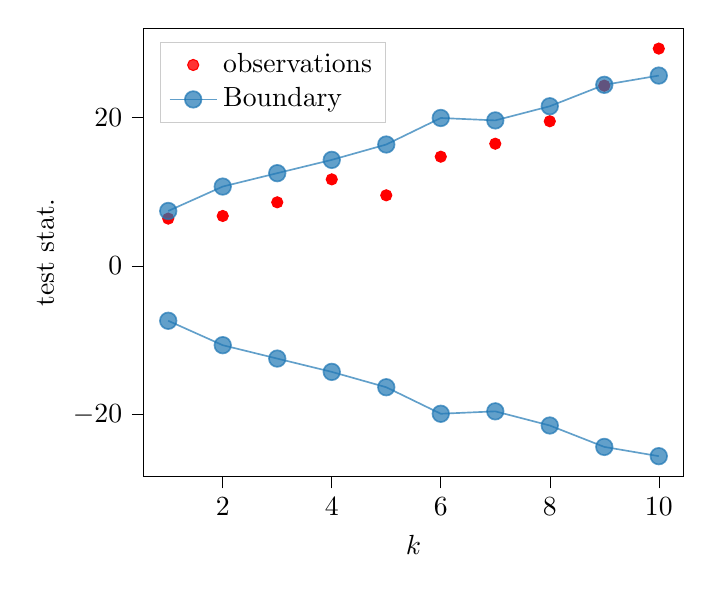
\begin{tikzpicture}

\definecolor{darkgray176}{RGB}{176,176,176}
\definecolor{lightgray204}{RGB}{204,204,204}
\definecolor{steelblue31119180}{RGB}{31,119,180}

\begin{axis}[
legend cell align={left},
legend style={
  fill opacity=0.8,
  draw opacity=1,
  text opacity=1,
  at={(0.03,0.97)},
  anchor=north west,
  draw=lightgray204
},
tick align=outside,
tick pos=left,
x grid style={darkgray176},
xlabel={\(\displaystyle k\)},
xmin=0.55, xmax=10.45,
xtick style={color=black},
y grid style={darkgray176},
ylabel={test stat.},
ymin=-28.399187576933, ymax=32.0363501618882,
ytick style={color=black}
]
\addplot [draw=red, fill=red, mark=*, only marks]
table{%
x  y
1 6.36951596974973
2 6.72822925865146
3 8.56830695564802
4 11.6617137827957
5 9.51291242818134
6 14.7166341712409
7 16.4678681124362
8 19.4958695694891
9 24.2934434420526
10 29.289280264669
};
\addlegendentry{observations}
\addplot [semithick, steelblue31119180, opacity=0.7, mark=*, mark size=3, mark options={solid}]
table {%
1 7.40127217830678
2 10.6925918052227
3 12.4974365317403
4 14.2892914784457
5 16.3614748247893
6 19.9360528087116
7 19.6101661169954
8 21.5183835738686
9 24.4040121396025
10 25.6521176797138
};
\addlegendentry{Boundary}
\addplot [semithick, steelblue31119180, opacity=0.7, mark=*, mark size=3, mark options={solid}, forget plot]
table {%
1 -7.40127217830678
2 -10.6925918052227
3 -12.4974365317403
4 -14.2892914784457
5 -16.3614748247893
6 -19.9360528087116
7 -19.6101661169954
8 -21.5183835738686
9 -24.4040121396025
10 -25.6521176797138
};
\end{axis}

\end{tikzpicture}
